\documentclass[10pt,twocolumn,letterpaper]{article}

\usepackage{cvpr}
\usepackage{times}
\usepackage{epsfig}
\usepackage{graphicx}
\usepackage{amsmath}
\usepackage{amssymb}

% Include other packages here, before hyperref.

% If you comment hyperref and then uncomment it, you should delete
% egpaper.aux before re-running latex.  (Or just hit 'q' on the first latex
% run, let it finish, and you should be clear).
\usepackage[pagebackref=true,breaklinks=true,letterpaper=true,colorlinks,bookmarks=false]{hyperref}

% \cvprfinalcopy % *** Uncomment this line for the final submission

\def\cvprPaperID{****} % *** Enter the CVPR Paper ID here
\def\httilde{\mbox{\tt\raisebox{-.5ex}{\symbol{126}}}}

% Pages are numbered in submission mode, and unnumbered in camera-ready
\ifcvprfinal\pagestyle{empty}\fi
\begin{document}

%%%%%%%%% TITLE
\title{Your Objective Is Wrong: Rethink Unsupervised learning of Optical Flow}

\author{First Author\\
Institution1\\
Institution1 address\\
{\tt\small firstauthor@i1.org}
% For a paper whose authors are all at the same institution,
% omit the following lines up until the closing ``}''.
% Additional authors and addresses can be added with ``\and'',
% just like the second author.
% To save space, use either the email address or home page, not both
\and
Second Author\\
Institution2\\
First line of institution2 address\\
{\tt\small secondauthor@i2.org}
}

\maketitle
%\thispagestyle{empty}

%%%%%%%%% ABSTRACT
\begin{abstract}
   The ABSTRACT is to be in fully-justified italicized text, at the top
   of the left-hand column, below the author and affiliation
   information. Use the word ``Abstract'' as the title, in 12-point
   Times, boldface type, centered relative to the column, initially
   capitalized. The abstract is to be in 10-point, single-spaced type.
   Leave two blank lines after the Abstract, then begin the main text.
   Look at previous CVPR abstracts to get a feel for style and length.
\end{abstract}

%%%%%%%%% BODY TEXT
\section{Introduction}

\subsection{Related Work}

\subsection{Novel Contribution}
We extend FlowNet~\cite{7410673} in this work, in summary our contributions are three folds. First, we proposed to combine traditional layered approach for optical flow estimation with deep learning. The proposed approach does not require pre-segmentation of images, instead, the separation of layers is automatically done during training the network. Second, a soft-masks module is proposed. This soft-masks module implements a channel-wise maxout operation among masks. As a result, the estimated optical flow will be separated to layers. each of which will contain optical flow that is estimated using a quadratic function. Third, we extend the FlowNet by adding the proposed soft-mask module in output layers, the resulting network is trained to compare with both supervised and unsupervised optical flow estimation approaches using neural networks. The empirical results show that the proposed network structure achieves comparable or lower error in each experimental group.

\section{Methodology}
The proposed approach and corresponding analysis will be introduced in this section.

\subsection{Annotation}
Given a pair of images $I_a, I_b \in \mathbb{R}^{H\times W\times C}$ as input, where $H, W$ and $C$ are height, width and channels of the input images. The proposed approach is going to estimate an optical flow field $\bold{u}, \bold{v} \in \mathbb{R}^{H\times W}$, where $\bold{u}$ and $\bold{v}$ are the horizontal and vertical components of the optical flow field to be estimated that transform image from $I_a$ to $I_b$. The original formulation of optical flow estimation is proposed by Horn and Schunck in~\cite{horn1981determining}. In classical formulation, an objective function is composed with a combination of a data term which makes a local constancy assumption of some image property and a spatial term that models how the flow is expected to vary across images. We write the classical optical flow objective function as:

\begin{equation}
\label{eqn: wrong obj}
E(\bold{u}, \bold{v}) = \sum_{i}^H\sum_{j}^W (I_1(i+u_{ij}, j+v_{ij}) - I_0(i, j))^2 + \varphi(\bold{u, v})
\end{equation}
where $\varphi(\bold{u}, \bold{v}))$ is a regularization term that constrains smoothness of optical flow. 

Nowadays, the above objective is still being used by many optical flow estimation using deep neural network based on unsupervised training framework~\cite{ahmadi2016unsupervised}\cite{ren2017unsupervised}\cite{DBLP:journals/corr/YuHD16}. We also use above objective when training our network and comparing with results of unsupervised methods. Experiments results are presented in Section~\ref{sec: evaluation}.

\begin{figure}[h]
\centerline{
\begin{tabular}{cc}
  \resizebox{0.089\textwidth}{!}{\rotatebox{0}{
  \includegraphics{Pic/PDF/NetworkStructure/Normal.pdf}}}
  &
  \resizebox{0.21\textwidth}{!}{\rotatebox{0}{
  \includegraphics{Pic/PDF/NetworkStructure/MaskModule.pdf}}}
  \\
  a. Normal output & b. Soft-masks module 
  \\
\end{tabular}}
\caption{An illustration of the structure of the proposed soft-masks module compared with normal linear optical flow output.}
\label{fig: soft-masks module}
\end{figure} 

\subsection{Soft-masks module}
FlowNet~\cite{7410673} is the first work that uses deep convolutional neural network for flow estimation. The network architecture used by FlowNet is very similar to classical structure of auto-encoder, where optical flows are generated using deconvolution at each scale level of the image pyramid. To refine estimation of the flows, shortcuts are built to connect layers of corresponding level in encoder and decoder. Given $x_{ij}\in \mathbb{R}^{k\times k \times c}$, where $k$ is kernel size and $c$ is number of channels, representing a feature vector inputted to output layer. FlowNet employs a linear activation to compute optical flow:

\begin{equation}
f_{ij} = x^T_{ij} W_{ij} + b_{ij}  
\end{equation}

Given actual optical flow field a nonlinear and piece-wise smooth representation of motions contained in images, using linear function to fit the flow field is less accurate. We introduce a soft-masks module in this paper. The proposed module can be used to replace the linear output of optical flow estimation. We will show that by using this module, we are able to separate optical flow field to multiple layers. Flow estimation in each layer is smooth and can be estimated using a quadratic function, which results in a more accurate and flexible optical flow estimation. 

An illustration of soft-masks module is shown in Figure~\ref{fig: soft-masks module}. The essential part of the soft-masks module is its dual-branch structure.

An illustration of soft-masks module is shown in Figure~\ref{fig: soft-masks module}. The essential part of the soft-masks module is its dual-branch structure.
An illustration of soft-masks module is shown in Figure~\ref{fig: soft-masks module}. The essential part of the soft-masks module is its dual-branch structure.An illustration of soft-masks module is shown in Figure~\ref{fig: soft-masks module}. The essential part of the soft-masks module is its dual-branch structure.

%\subsection{Correct Objective Function}
%\label{subsec: correct obj}
%For existing works \cite{ahmadi2016unsupervised}\cite{ren2017unsupervised}\cite{DBLP:journals/corr/YuHD16}, unsupervised learning of optical flow is achieved by using a network framework that combines FlowNet \cite{7410673} and Spatial Transformation Network (STN) \cite{NIPS2015_5854}. Given a fact that image transformation is a reverse mapping in STN, so, the optical flow is actually transforming $I_1$ in this case. Existing works follow a same pattern and define their objective function as following:
%
%It is helpful to think about a fact that how optical flow exactly transforms image $I_1$ in reverse mapping in Eqn.\ref{eqn: wrong obj}. Suppose a new image denoted as $I^*$ will be produced by transforming $I_1$ using the optical flow. The expression $I_1(i+u_{ij}, j+v_{i,j})$ in Eqn.\ref{eqn: wrong obj} actually means the pixel $I_1(i+u_{ij}, j+v_{ij})$ will  will get \textit{copied} and \textit{moved} by flow vector $(u_{ij}, v_{ij})$ to pixel $I^*(i, j)$ in image $I^*$. Then one question raises up that what happens to pixel $I^*(i+u_{ij}, j+v_{ij})$ in image $I^*$, is it gauranteed that there is always a pixel in image $I_0$ will get copied to $I^*(i+u_{ij}, j+v_{ij})$? The answer actually depends on optical flows at other pixels. For better understanding, an illustration showing the transformation caused by optical flow is given in Fig.\ref{fig: demo wrong obj}.
%
%\begin{figure}[h]
%\centerline{
%\begin{tabular}{cc}
%  \resizebox{0.21\textwidth}{!}{\rotatebox{0}{
%  \fbox{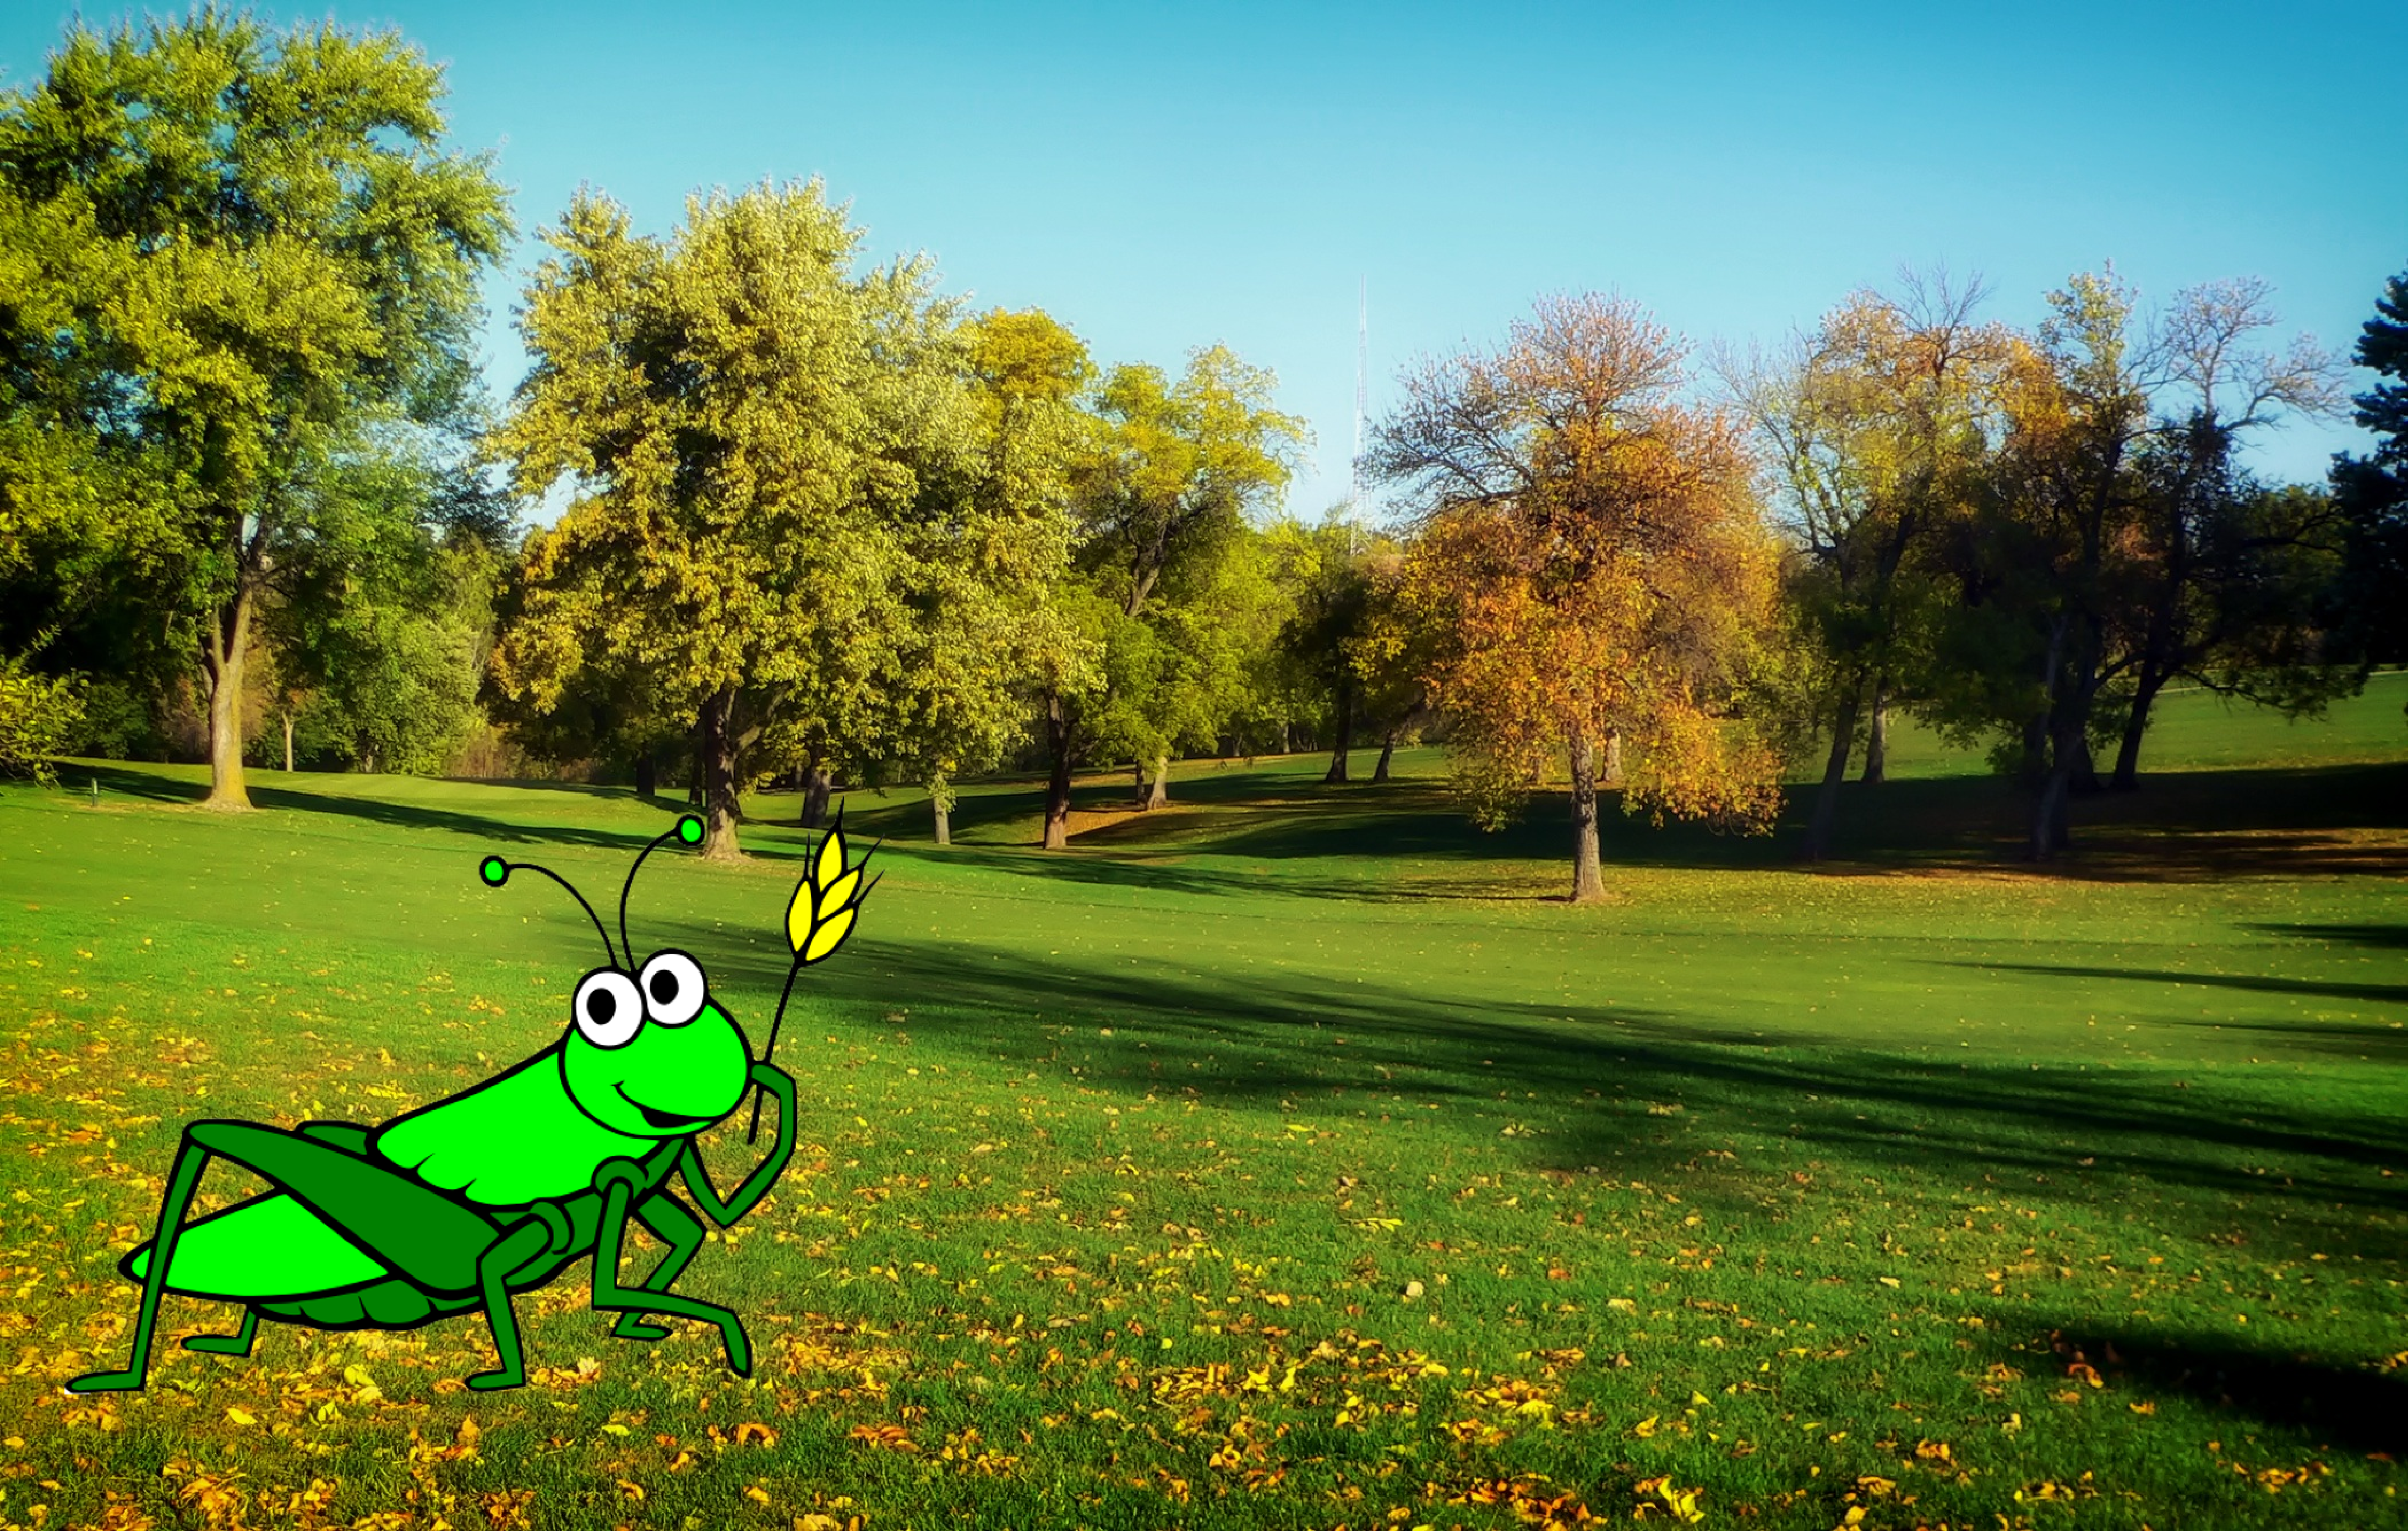
\includegraphics{Pic/PDF/Demo_wrong_obj/hopper_demo_src.pdf}}}}
%  &
%  \resizebox{0.21\textwidth}{!}{\rotatebox{0}{
%  \fbox{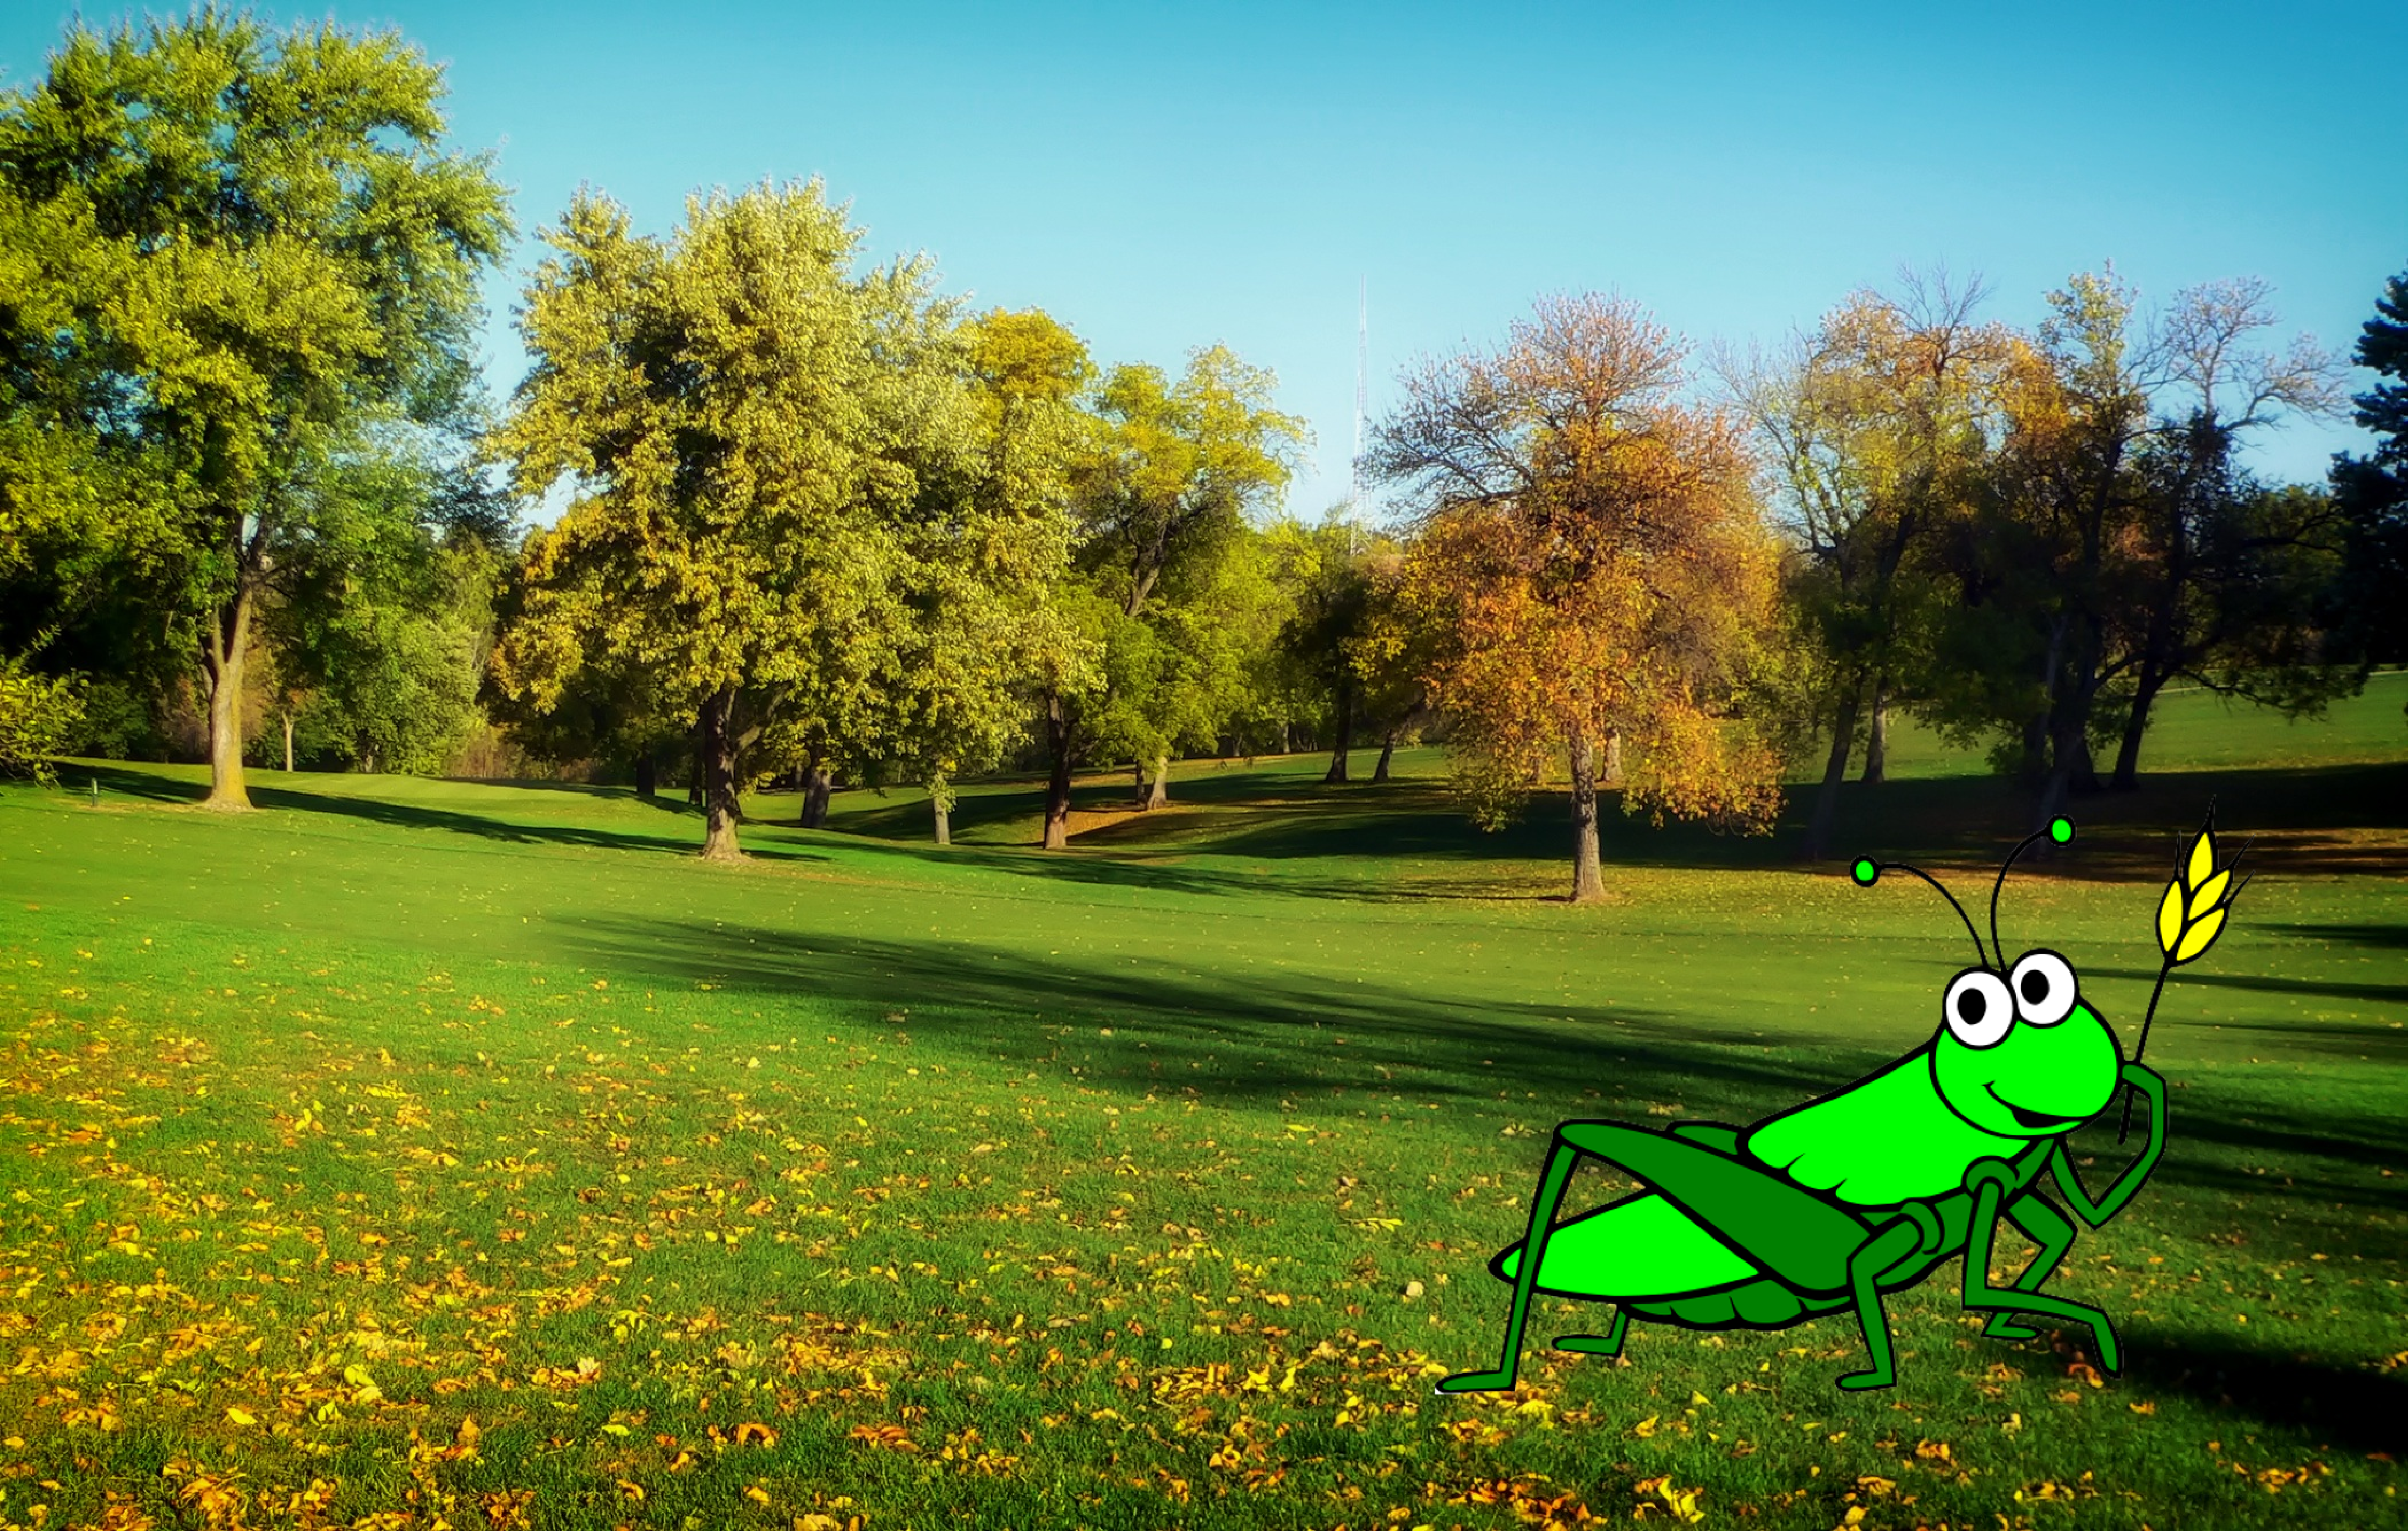
\includegraphics{Pic/PDF/Demo_wrong_obj/hopper_demo_dst.pdf}}}}
%  \\
%  a. $I_0$ & b. $I_1$
%  \\
%  \resizebox{0.21\textwidth}{!}{\rotatebox{0}{
%  \fbox{\includegraphics{Pic/PDF/Demo_wrong_obj/hopper_demo_flow.pdf}}}}
%  &
%  \resizebox{0.21\textwidth}{!}{\rotatebox{0}{
%  \fbox{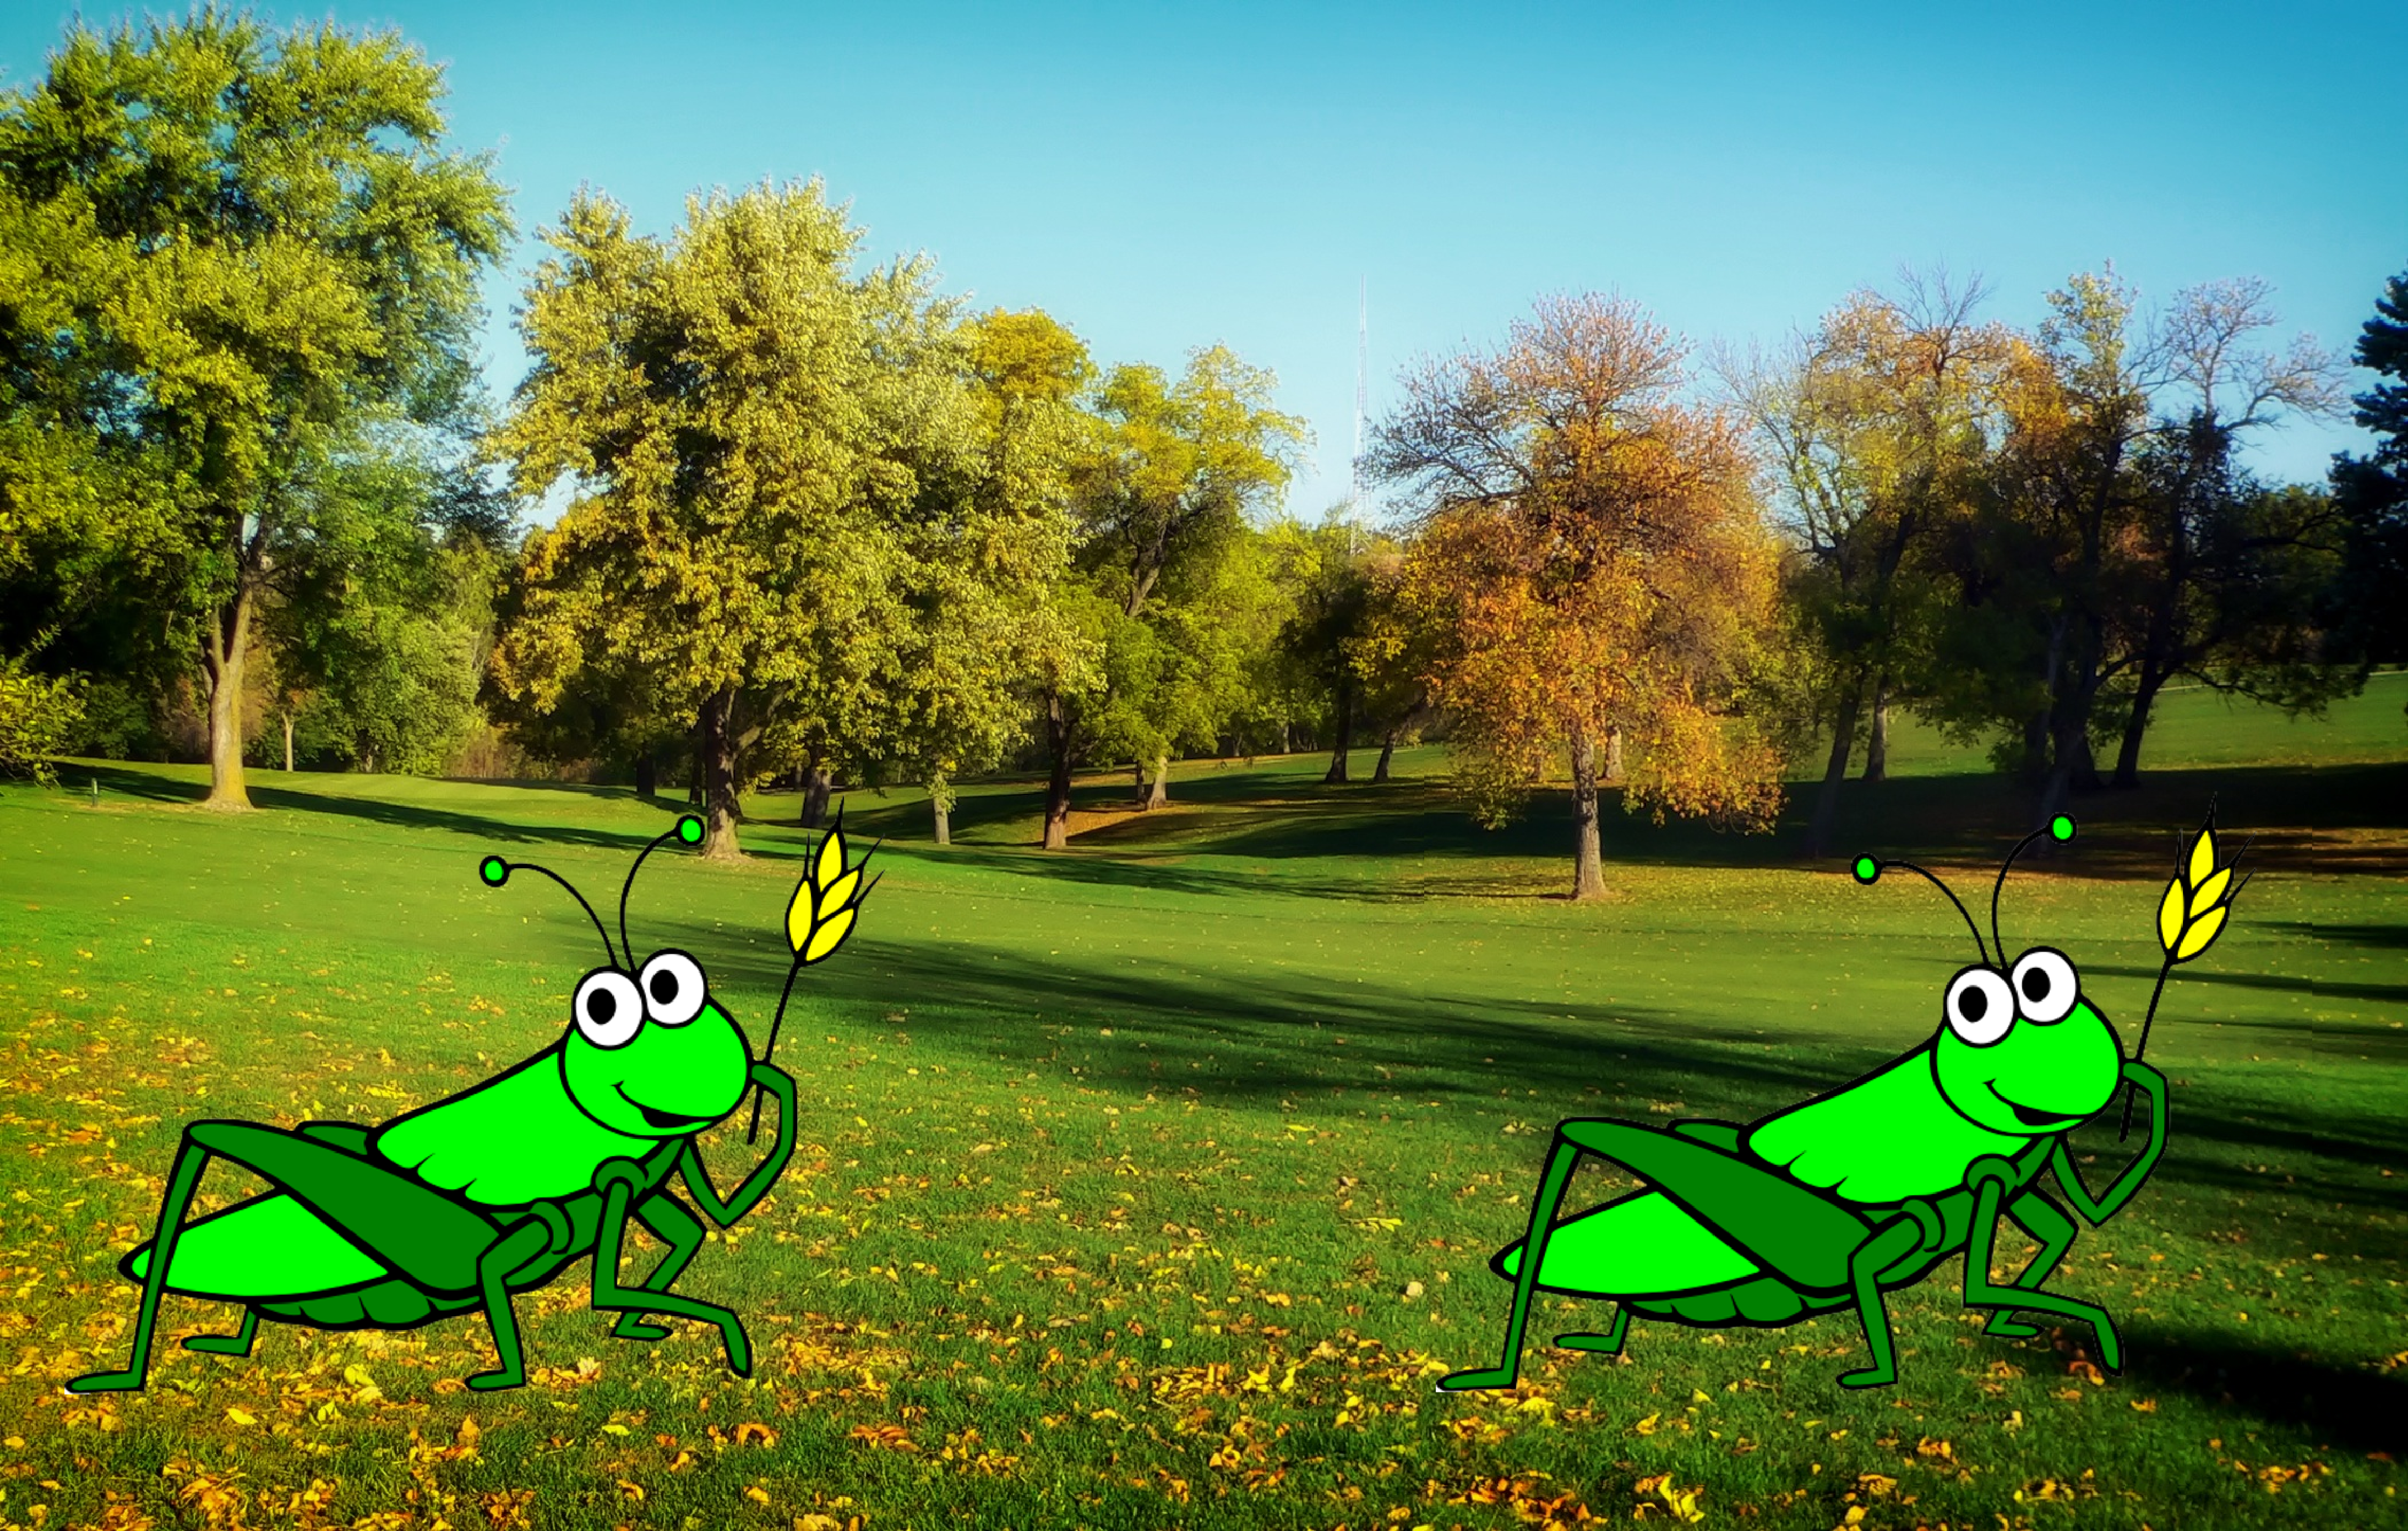
\includegraphics{Pic/PDF/Demo_wrong_obj/hopper_demo_true_bkwd.pdf}}}}
%  \\
%  c. Flow & d. $I^*$
%\end{tabular}}
%\caption{Illustration of image transformation as a result of reverse mapping using optical flow.}
%\label{fig: demo wrong obj}
%\end{figure} 
%
%In Fig.\ref{fig: demo wrong obj}, a grasshopper is going to hop from left in $I_0$ to right in $I_1$ with static background in both images. Fig.\ref{fig: demo wrong obj}c shows the ground truth optical flow from $I_0$ to $I_1$, in which only area of grasshopper gets non-zero flow. Now, let us suppose $I^*$ starts as an empty image and we first focus on the area of grasshopper where optical flow is not zero. Given a pixel location $(i, j)$ in the grasshopper area and a flow vector at this pixel $(u_{ij}, v_{ij})$, because of transformation, we will have $I^*(i, j)=I_1(i+u_{ij}, j+v_{ij})$, which moves grasshopper from right side in $I_1$ to left side in $I^*$. Then let us consider background areas with no optical flow, following the same rule, we will have $I^*(i, j)=I_1(i+0, j+0)$. That is to say, the background area in $I_1$ including the grasshopper will be exactly copied to $I^*$. As a result, we are able to see two grasshoppers in $I^*$. 
%
%It could be known from this illustration that, it is not necessarily true that $I^*$ will be identical to $I_0$ even being transformed using true optical flow. Using Eqn.\ref{eqn: wrong obj} as an objective thus will not gaurantee that network is able to learn a correct optical flow. Because using $I_0$ as target image, the training process will force optical flow to be generated to produce $I^*$ which is exactly the same to $I_0$. As a result, the estimation of optical flow could easily be wrong. So, in this paper, we argue that, under the unsupervised optical flow learning framework, using $I_0$ as reference image is wrong. Instead the correct reference image is $I^*$, the learning of which requires accessing to the ground truth optical flow. 

\subsection{Target Image Estimation Network}
\label{subsec: target image net}

\subsection{Flow Estimation Network}
\label{subsec: flow net}

\section{Empirical Evaluation}
\label{sec: evaluation}

\subsection{Datasets}

\subsection{Training Details}

\subsection{Results}

\section{Discussion and Summary}

{\small
\bibliographystyle{ieee}
\bibliography{mybib}
}

\end{document}
